\csname documentclass\endcsname[../main.tex]{subfiles}
\begin{document}
\chapter{Evaluation}\label{chapter-4}

In this chapter, we evaluate the performance of our RLCEM, and compare it 
against existing greedy intervention policies. RLCEM is a CEM augmented with an RL agent
to learn a non-greedy intervention policy, and trained according to Section~\ref{method:rlcem}.
We compare RLCEM to our baseline, 
including two of the known best-performing~\cite{intcem} 
greedy intervention policies
IntCEM and CooP.


All experiments in this chapter
are conducted across three trials, where we report the mean
and standard deviation. This helps make our results more statistically significant and reduces the errors
that arise from randomness.

\section{Baseline Intervention Policies}
To evaluate the performance of RLCEM, we compare RLCEM to existing greedy intervention policies IntCEM, and CooP.
 IntCEM learns a greedy intervention policy
by mimicking the behaviour of an optimal greedy policy,
and CooP is a heuristic-based greedy intervention policy
that selects concepts to intervene based on its associated uncertainty
and importance score. As mentioned in
Section~\ref{background:coop}, CooP uses a weighted average
of three scores, and thus we perform a grid search for the weight 
of these three weights, and select the combination of weights with the best performance.
We also compare RLCEM to Random, a policy that selects
random concepts to intervene on.
We compare the RLCEM intervention policy against these three baseline intervention policies.

\section{Models and Datasets}\label{method:datasets}
% Brief description of each of these datasets and what they are each used for.
% Leave full description to be in appendix.
% Talk about concept groups
% Talk about subsampling
To evaluate the performance of our RLCEM model,
we follow Zarlenga et al.~\cite{intcem} and select the datasets MNIST-ADD and CUB for 
our experiments. 
% Since these datasets have different input image sizes,
% we use $\mathbf{x} \to \mathbf{c}$ models 
% are slightly different, which we directly select the same 
% models as Zarlenga et al.~\cite{intcem}
% for a fair comparison. 
We use the same $\mathbf{x} \to \mathbf{c}$
and $\mathbf{c} \to \mathbf{y}$ models
for RLCEM and the baseline IntCEM to ensure the results reflect a fair comparison 
of the learnt intervention policy, which we follow from Zarlenga et al.~\cite{intcem}.
% Additionally for most of our ablation studies,
% we conduct it on MNIST-ADD due to its straightforwardness.
For both datasets, 20\% of the training dataset is selected
as a validation dataset to monitor
the performance of the model during training. This is used for hyperparameter
selection and early stopping to prevent over-fitting. A summary of the two
datasets used can be found in Table~\ref{table:datasets}.

\subsection{MNIST-ADD}
MNIST-ADD is a dataset created from 
the MNIST~\cite{mnist} dataset. 
The MNIST dataset consists of hand-written digits from 0 to 9,
which are black-and-white images with sizes $1 \times 28 \times 28$.
MNIST-ADD samples
12 images from the MNIST dataset as input $\mathbf{x}$,
with concepts corresponding to the values of each of the input images.
To model concept-incompleteness in real life datasets~\cite{cem},
which is when the 
concept annotations do not contain all
concepts relevant to predicting the label, we only select the concepts corresponding to 8
of the input images, ensuring that the same conceps are selected across
all samples. This produces $54$ concepts which are then grouped into 8 
mutually-exclusive concept groups corresponding to images.
The label for each MNIST-ADD sample
is a binary label $\mathbf{y}$ corresponding to whether or not the sum of the input
12 images is greater than half of the possible maximum value.
The MNIST-ADD dataset consists of 
 10,000 training samples and 10,000 test samples, formed by choosing
each of the 12 input images randomly from the MNIST training and testing
datasets respectively.

For this task, we use a ResNet-18~\cite{resnet} backbone for the $\mathbf{x} \to \mathbf{c}$
model with its output linear layer modified to 54 activations, corresponding
to the 54 concepts. The ResNet-18 backbone consists of 18 residual layers,
each containing two convolutional layers with batch normalization and non-linear
activation functions, and is a popular backbone for image-related tasks.
The $\mathbf{c} \to \mathbf{y}$ model is an MLP with \{128, 128\} hidden
layer activations, and forwards the 54 predicted concepts to predict the binary label.
As it is a binary task, we use AUC instead of accuracy to measure the performance 
as it is less sensitive to class imbalances 
and classification thresholds.

\subsection{CUB}

CUB~\cite{cub} is a real-life concept-annotated dataset that identifies birds.
The input $\mathbf{x}$ consist of $3 \times 299 \times 299$ coloured images of 
 birds, and output $\mathbf{y}$ is a label corresponding to the species of the bird.
There are 
112 concepts 
representing features of birds such as their colour, shape, etc.,
which are then grouped into 28 concept groups according
to Zarlenga et al~\cite{intcem}. We further group these
into 7 different concept groups by their
semantic similarity for easy visualization and a better comparison
with MNIST-ADD. This also allows us to use the same RL models across datasets
as the size of the action space is simiar. There are 
5,994 training samples and 5,794 testing samples.

For this dataset, we use a ResNet-34~\cite{resnet} backbone for the 
$\mathbf{x} \to \mathbf{c}$
model with its output linear layer modified to 112 activations, corresponding
to the 112 concepts. The ResNet-34 uses the same layers as ResNet-18
with more layers deigned to process larger and more complicated images,
which we select due to the larger and more complex images in the CUB dataset.
The $\mathbf{c} \to \mathbf{y}$ model is an MLP with \{128, 128\} as the hidden
layer activations, and forwards the 112 predicted concepts to predict the label out of 200 classes.
% \subsection{CelebA}

% CelebA is another synthetic dataset constructed from 
% the popular CelebA dataset, a dataset that identifies celebrity face attributes.

\begin{table}
    \centering
    \renewcommand{\arraystretch}{1.5}
    \begin{tabular}{c|cc}
    % Dataset & Training Samples & Test Samples & Input Size & Concepts (k) & 
    % Concept Groups (n) & Output classes \\
    % \hline
    % MNIST-ADD & 10,000 & 10,000 & [12,28,28] & 54 & 8 & 2 \\
    % CUB & 5,994 & 5,794 & [3,299,299] & 112 & 28 & 200

    Dataset & MNIST-ADD & CUB \\
    \hline
    Training Samples & 10,000 & 5,994 \\
    Testing Samples & 10,000 & 5,794 \\
    Input Size & [12,28,28] & [3,299,299]\\
    Concepts (k) & 54 & 112 \\
    Concept Groups (n) & 8 & 7 \\
    Output classes & 2 & 200
    \end{tabular}
    \caption{The datasets and tasks used in this project.}
    \label{table:datasets}
\end{table}

More details on the datasets used can be found at Appendix~\ref{appendix:datasets}.

% \subsection{Evaluating Performance}


\subsection{Reinforcement Learning agent Model}
We adopt the same MLP for 
both the Actor and Critic model in the RL agent, 
using the same MLP structure as that in the IntCEM intervention policy model,
but increase the number of activations in the hidden layers
 from \{128, 128, 64, 64\} to \{512, 512, 256, 256\} as
 our task of learning a non-greedy policy is more complex.
 The RL agent needs to learn 
 $O(n^2)$ sub-tasks instead of $O(n)$, as there are $O(n)$ 
steps per budget for $O(n)$ different budgets.
 The same model is used
 for all datasets as the number of concept groups for intervention,
 which corresponds to the action space,
 is similar. 
%  We find that increasing the number of hidden layer neurons
%  in the MLP used by 
%  IntCEM to \{512, 512, 256, 256\} does not have any noticeable improvements
%  to the intervention performance
%  on a validation set.
% \begin{table}
%     \centering
%     \begin{tabular*}{width}[pos]{cols}
        
%     \end{tabular*}
%     \caption{Performance of GreedyOptimal vs TrueOptimal }
% \end{table}

\section{Surrogate Models}\label{eval:surrogate}

We then look into the training of the 
surrogate models, which are used to model the conditional
likelihoods $p(\mathbf{c}_u \mid \mathbf{c}_o, \mathbf{y})$ and used 
to provide intermediate rewards to the RL agent.
As mentioned in Section~\ref{method:surrogate}, 
we train the AC Flow model
using a negative log likelihood loss and a cross
entropy loss, using random samples of $\mathbf{c}_o$ and 
$\mathbf{c}_u$ that are subsets of the overall concepts.
The trained AC Flow model
will be frozen and used in the RLCEM model
to provide intermediate rewards to the RL agent.

To evaluate the performance of a trained 
AC Flow model, we look at 
its negative log likelihood and its accuracy on a validation set.
This is the accuracy of predicting 
the label $\hat{\mathbf{y}}$ 
based on the class with the highest likelihood for 
concepts in the dataset, 
given by
\[\hat{\mathbf{y}} = \mathrm{\mathop{argmax}}_{\mathbf{y}} \;
p( \mathbf{y} \mid \mathbf{c}_o)\]
whereas the negative log likelihood (NLL) is the 
negative log likelihood of 
$p(\mathbf{c}_u \mid \mathbf{c}_o, \mathbf{y})$
for concepts $\mathbf{c}_u$ and $\mathbf{c}_o$ 
present in the validation dataset.
%  We stop training if the validation loss
% does not improve over several epochs, a common tactic used
% to avoid over-fitting.

\begin{figure}[!h]
    \centering
    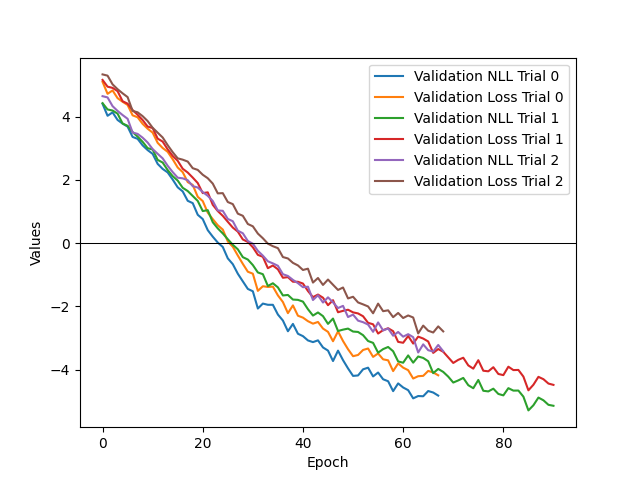
\includegraphics[width=0.7\textwidth]{figs/evaluation/mnist_acflow_no_val_accuracy_no_l2_loss_nll.png}
    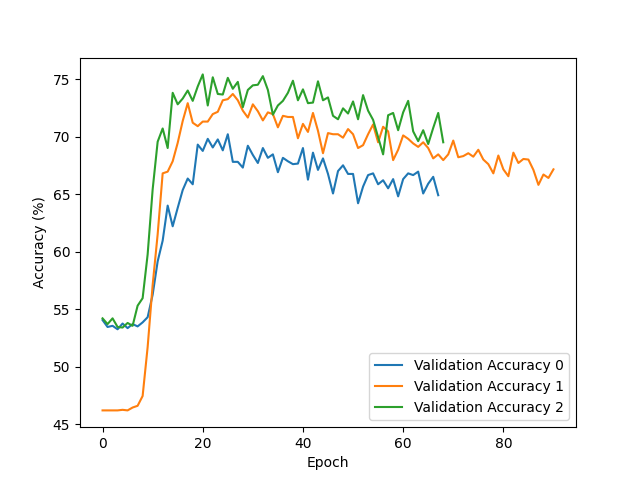
\includegraphics[width=0.7\textwidth]{figs/evaluation/mnist_acflow_no_val_accuracy_no_l2_accuracy.png}
    \caption{
        Performance on Validation Set when training an AC Flow model
        on the MNIST-ADD dataset across 3 trials.
        Top: Validation NLL and loss. Bottom: Validation Accuracy.
    }
    \label{fig:mnist-acflow-no-val-accuracy-no-l2-loss}
\end{figure}

Figure~\ref{fig:mnist-acflow-no-val-accuracy-no-l2-loss} shows the 
validation results when training an AC Flow model
on the MNIST-ADD dataset, using a learning-rate of 1e-6.
%  and 
% early stopping if validation loss does not improve over 5 epochs.
A large issue that we observe is that the validation loss
keeps decreasing and there is no limit to stop it.
This is because the model learns to output the log likelihoods 
of $p(\mathbf{c}_u \mid \mathbf{c}_o, \mathbf{y})$, and the underlying
model is a Gaussian Mixture Model which learns to output
a probability density at each value. While these probability densities
tells us about the likelihoods,
they are not probability values within $[0,1]$. A likelihood value greater than 1 translates to a positive likelihood,
thus the log likelihood can fall outside of $[-\infty, 0]$,
translating to a negative NLL and negative los.
% it does not output an absolute probability with values in Therefore
% the  and contain 
% positive values, which is translated to a negative NLL and negative loss.
The model learns to output larger and larger
values for the more probable likelihoods, and the NLL keeps decreasing
below 0, as there is no upper limit to the values the likelihoods can take.
% and the model does not appear to be able to stop as there is no
% upper limit to the values it can output (and no lower limit to the NLL and hence
% loss).
 At the same time the validation accuracy stops improving
 much quicker and then deteriorates, indicating that the model is over-fitting
long before validation loss starts to converge.
As a result, we use the validation accuracy as an early stopping
metric to prevent over-fitting. This helps ensure that 
the model learns about the underlying distribution and 
the log likelihood values accurately reflect the likelihood 
of concepts, which is 
shown from the validation accuracy, while preventing 
the output log likelihood values from growing endlessly, which
as we can see in Section~\ref{eval:rlcem-performance}, 
leads to other issues.

\section{Evaluating RLCEM}\label{eval:rlcem-performance}

We implement RLCEMs according to Section~\ref{method:rlcem},
implementing the Reinforcement Learning environment using the 
open-source
Gymnasium~\cite{gymnasium} interface. This allows our RLCEM to be integrated
 with the Gymnasium RL ecosystem, and our implementation
to be available to the research community for further research in 
RL-based intervention policies.

We train RLCEMs and evaluate them on the datasets MNIST-ADD and CUB, 
comparing them against three other intervention policies:
IntCEM, CooP, and Random. While IntCEM is evaluated on the
CEM learnt together with the IntCEM policy,
we evaluate CooP and Random on the CEM learnt 
with the RL based policy. This is to ensure a fair comparison
with the RLCEM policy.

\subsection{Training Hyperparameters}

The hyperparameters used for training IntCEM and an RLCEM are similar,
consisting of the weights of the losses in the overall loss equation
\[\mathcal{L} = \lambda_{\text{concept}} \mathcal{L}_{\text{concept}}
+  \lambda_{\text{label}} \mathcal{L}_{\text{label}}
+  \lambda_{\text{intervention}} \mathcal{L}_{\text{intervention}}\]
The hyperparameters used also include
the label loss discount factor for interventions $\gamma$,
and other common hyperparameters for Machine Learning such as learning rate
and batch size.
We follow the recommended hyperparameters 
for IntCEM from Zarlenga et al.~\cite{intcem}. 
Due 
to similarities between IntCEM and RLCEM, we re-use
the same loss weights except $\lambda_{\text{intervention}}$,
the weight of the loss used to train the intervention policy model.
For RLCEM, we search over $\lambda_{\text{intervention}} \in [0.2, 1, 5]$, and select based on validation
intervention performance.
We train all models using the Adam~\cite{adam} optimizer, with learning rates
from [1e-3, 1e-4, 1e-5], and 
batch size to fit the hardware we use.
We train for a maximum of 300 epochs,
and stop training if the validation loss stops improving over 15 epochs
to prevent over-fitting.
A summary of the hyperparameters used is shown in 
Table~\ref{table:hyperparameters}.

\begin{table}[!ht]
    \centering
    \renewcommand{\arraystretch}{1.5}
    \begin{tabular}{c|cccc}
        Hyperparameter & \multicolumn{2}{c}{IntCEM} & \multicolumn{2}{c}{RLCEM} \\
        \hline
        Task & MNIST-ADD & CUB &
        MNIST-ADD & CUB \\ 
        Learning Rate & 1e-5 & 1e-4 & 1e-5 & 1e-4 \\
        \hline
        $\lambda_{\text{concept}}$ & \multicolumn{2}{c}{5} & \multicolumn{2}{c}{5}\\
        $\lambda_{\text{label}}$ & \multicolumn{2}{c}{1} & \multicolumn{2}{c}{1}\\
        $\lambda_{\text{intervention}}$ & \multicolumn{2}{c}{5} & \multicolumn{2}{c}{1}\\
        $\gamma$ & \multicolumn{2}{c}{1.1} & \multicolumn{2}{c}{1.1} \\
        Policy Model Activations & \multicolumn{2}{c}{\{128, 128, 64, 64\}}
        &  \multicolumn{2}{c}{\{512, 512, 256, 256\}} \\
    \end{tabular}
    \caption{Training Hyperparameters used to train IntCEM and RLCEM for the 
    two tasks MNIST-ADD and CUB. }
    \label{table:hyperparameters}
\end{table}

\subsection{MNIST-ADD}

% After training the AC Flow model on the MNIST-ADD dataset 
% as illustrated in the previous section, we train RLCEM by 
% using the
% pretrained AC Flow model to provide intermediate rewards equal to 
% the increase in information to the target as mentioned in 
% Section~\ref{method:rlcem}.
RLCEM's test intervention performance  against 
existing intervention policies is shown in
Figure~\ref{fig:mnist-performance-no-l2},
and the performance across quartiles of interventions is shown in Table~\ref{table:mnist-performance-no-l2}.
We see that 
% barring the first and last intervention performance,
% where all non-greedy and greedy intervention policies perform similarly,
RLCEM outperforms all of IntCEM, CooP and Random, yielding a 
higher AUC under the same number of interventions. It also achieves similar or better intervention performance with 25\% less groups
intervened.
When no interventions are performed, 
RLCEM has a similar performance to 
IntCEM, showing that the intervention performance
increase does not come at the expense of un-intervened performance.
This is expected as the base CEMs are trained 
in a similar fashion. Additionally, IntCEM outperforms Random
 at first but the performance of 
IntCEM degrades as interventions increase,
also supports the hypothesis that greedy intervention policies 
may learn
sub-optimal policies for different budgets, especially for larger
 budgets.
RLCEM combines the strategy of directly learning a policy from IntCEM,
and the uncertainty-based strategy of CooP, and learns an intervention policy
that dynamically balances between them based on the budget.
% Intuitively,
% while an optimal policy for a smaller budget may try to correct 

\begin{figure}[!ht]
    \centering
    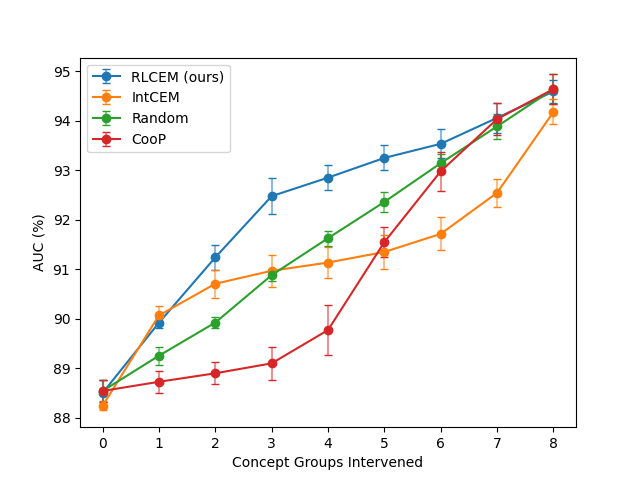
\includegraphics[width=0.9\textwidth]{figs/evaluation/mnist_rlcem_performance.png}
    \caption{
        Intervention AUC (\%) of RLCEM intervention
    policy compared to existing intervention policies on MNIST-ADD.
    }
    \label{fig:mnist-performance-no-l2}
\end{figure}


\begin{table}[!ht]
    \centering
    \renewcommand{\arraystretch}{1.5}
    \begin{tabular}{c|ccccc}
        \begin{tabular}{@{}c@{}}Concept Groups \\ Intervened\end{tabular} & RLCEM (Ours) & IntCEM & CooP & Random \\
    \hline
    % $0\%$ & $\mathbf{88.2} \pm 0.3$ & $\mathbf{88.24} \pm 0.09$ & $\mathbf{88.24} \pm 0.09$ & $\mathbf{88.24} \pm 0.09$ \\
    % $25\%$ & $\mathbf{91.1} \pm 0.4$ & $\mathbf{90.7} \pm 0.3$ & $88.7 \pm 0.2$ & $89.55 \pm 0.08$ \\
    % $50\%$ & $\mathbf{93.2} \pm 0.2$ & $91.1 \pm 0.3$ & $91.1 \pm 0.2$ & $91.24 \pm 0.07$ \\
    % $75\%$ & $\mathbf{94.0} \pm 0.2$ & $91.7 \pm 0.3$ & $93.4 \pm 0.2$ & $92.7 \pm 0.2$ \\
    % $100\%$ & $\mathbf{94.5} \pm 0.4$ & $\mathbf{94.2} \pm 0.3$ & $\mathbf{94.2} \pm 0.3$ & $\mathbf{94.2} \pm 0.3$ \\
    $0\%$ & $\mathbf{88.5} \pm 0.2$ & $88.24 \pm 0.09$ & $\mathbf{88.5} \pm 0.2$ & $\mathbf{88.5} \pm 0.2$ \\
$25\%$ & $\mathbf{91.2} \pm 0.2$ & $90.7 \pm 0.3$ & $88.9 \pm 0.2$ & $89.9 \pm 0.1$ \\
$50\%$ & $\mathbf{92.9} \pm 0.3$ & $91.1 \pm 0.3$ & $89.8 \pm 0.5$ & $91.6 \pm 0.1$ \\
$75\%$ & $\mathbf{93.5} \pm 0.3$ & $91.7 \pm 0.3$ & $93.0 \pm 0.4$ & $93.1 \pm 0.2$ \\
$100\%$ & $\mathbf{94.6} \pm 0.2$ & $94.2 \pm 0.3$ & $\mathbf{94.6} \pm 0.2$ & $\mathbf{94.6} \pm 0.2$ \\
    \end{tabular}
    \caption{Intervention AUC (\%) of RLCEM intervention
    policy compared to existing intervention policies on MNIST-ADD,
    across quartiles of interventions performed.
    Higher is better. We highlight the 
    best performing policy in each row and values within 1 standard deviation.}
    \label{table:mnist-performance-no-l2}
\end{table}

We have successfully shown that RLCEM is able to find a better 
policy than CooP and Random, since all these policies were tested
on the same CEMs. However despite RLCEM outperforming 
IntCEM in intervention performance, to analyze the RLCEM and IntCEM 
policies we need to take into account the sensitivities 
to interventions, as these 
two policies are tested on their respective trained CEMs, and the performance
difference could be attributed to the CEM rather than the policy. To test 
the sensitivity of RLCEM and IntCEM to interventions, we compare 
applying Random interventions to the two trained CEMs.

\begin{figure}[!h]
    \centering
    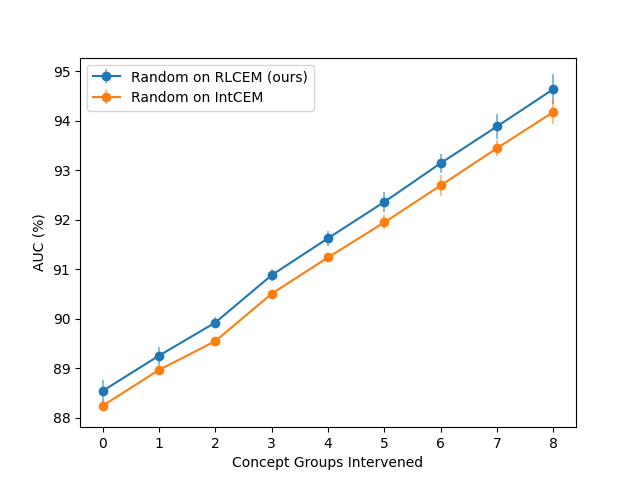
\includegraphics[width=0.9\textwidth]{figs/evaluation/mnist_performance_random_off.png}
    \caption{
        Intervention AUC (\%) of Random Interventions on RLCEM and IntCEM.
    }
    \label{fig:mnist-random-off}
\end{figure}

Figure~\ref{fig:mnist-random-off} shows the intervention performance of Random
on RLCEM and IntCEM. We see that the two have very similar intervention performances,
both exhibiting a linear increase in AUC as the number of interventions increase.
This shows that they have very similar sensitivities to intervention, which 
allows us to draw the conclusion that RLCEM learns a more optimal
intervention policy 
than IntCEM for different budgets.

% \begin{table}
%     \centering
%     \renewcommand{\arraystretch}{1.5}
%     \begin{tabular}{c|cc}
%         \begin{tabular}{@{}c@{}}Concept Groups \\ Intervened\end{tabular} & Random on RLCEM & Random on IntCEM \\
%     \hline
%     % $0\%$ & $\mathbf{88.2} \pm 0.3$ & $\mathbf{88.24} \pm 0.09$ & $\mathbf{88.24} \pm 0.09$ & $\mathbf{88.24} \pm 0.09$ \\
%     % $25\%$ & $\mathbf{91.1} \pm 0.4$ & $\mathbf{90.7} \pm 0.3$ & $88.7 \pm 0.2$ & $89.55 \pm 0.08$ \\
%     % $50\%$ & $\mathbf{93.2} \pm 0.2$ & $91.1 \pm 0.3$ & $91.1 \pm 0.2$ & $91.24 \pm 0.07$ \\
%     % $75\%$ & $\mathbf{94.0} \pm 0.2$ & $91.7 \pm 0.3$ & $93.4 \pm 0.2$ & $92.7 \pm 0.2$ \\
%     % $100\%$ & $\mathbf{94.5} \pm 0.4$ & $\mathbf{94.2} \pm 0.3$ & $\mathbf{94.2} \pm 0.3$ & $\mathbf{94.2} \pm 0.3$ \\
%     $0\%$ & $88.5 \pm 0.2$ & $88.24 \pm 0.09$ \\
%     $25\%$ & $89.9 \pm 0.1$ & $89.55 \pm 0.08$ \\
%     $50\%$ & $91.6 \pm 0.1$ & $91.24 \pm 0.07$ \\
%     $75\%$ & $93.1 \pm 0.2$ & $92.7 \pm 0.2$ \\
%     $100\%$ & $94.6 \pm 0.3$ & $94.2 \pm 0.3$ \\
%     \end{tabular}
%     \caption{Intervention AUC (\%) of Random Interventions on RLCEM and IntCEM,
%     across quartiles of interventions performed. Higher is better.}
%     \label{table:mnist-random-off}
% \end{table}

\subsection{CUB}

We evaluate the performance of RLCEM against existing 
greedy intervention policies on CUB. However, an important issue 
we faced was loss exponentially increasing, 
in particular the value loss for the Critic model of the
RL agent, as seen in Figure~\ref{fig:cub-v-loss-spike} where the y-axis is 
logarithmic.


\begin{figure}[!h]
    \centering
    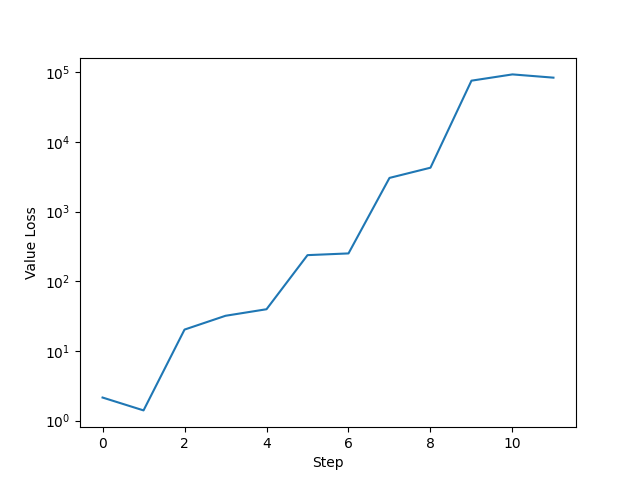
\includegraphics[width=0.9\textwidth]{figs/evaluation/cub_v_loss_spike.png}
    \caption{
        Value Loss of RLCEM when trained on CUB,
        y-axis is logarithmic scale.
        The value loss increases exponentially with steps, 
        and becomes very large, which is undesirable.
    }
    \label{fig:cub-v-loss-spike}
\end{figure}

The reason for this is the outputs of the AC Flow model
are too large.
In Section~\ref{eval:surrogate} we mentioned measures we took to prevent
the likelihood values outputted by the AC Flow model from being too large.
However, CUB has a large number of concepts and 
the relationships between concepts is more straightforward,
where features can be grouped by
whether they appear on the same bird species.
This is not the case in MNIST-ADD as the distribution of concepts corresponding to 
different 
digits are independent of each other.
The model for CUB quickly converges and the outputted log likelihoods 
for concepts increase rapidly leading to an exponential increase 
in outputted likelihoods. This means that the rewards for the RL agent
are also very large, which result in enormous value losses.
Not only does this damage the model's ability to learn
as the large loss values and updates cause instability and numerical
issues in training,
it also means that the intermediate rewards will overpower the final reward,
rendering it useless in training the model.
This means that the agent only learns to 
maximize expected information gain rather than
also maximizing the post-intervention performance,
which is our main goal.
Since the issue is with the output of the AC Flow model
which is used as rewards, common methods to prevent loss spiking
and exploding gradients,
such as clipping the gradient or losses, did not alleviate the problem.
Normalizing the outputs is also infeasible as that would require
normalizing over all concept and label combinations in 
$p(\mathbf{c}_u \mid \mathbf{c}_o, \mathbf{y})$,
which is intractable.


% Another supporting statistic for this is that the validation 
% accuracy of the AC Flow model for CUB reaches higher than $85\%$ out of 
% 200 classes, whereas the accuracy of the AC Flow model of MNIST-ADD is only around
% $70\%$ for a binary task.

In order to solve this problem, we add a penalty 
to the loss term of the AC Flow model to penalize
large log likelihoods. As mentioned in Section~\ref{method:training-surrogate-model},
we add an $\ell_2$ penalty
\[\lambda_{\ell_2} \left ( \log^2 p(\mathbf{c}_u, \mathbf{c}_o \mid \mathbf{y}) + 
\log^2 p(\mathbf{c}_o \mid \mathbf{y}) \right )\]
to the loss, and we try to set $\lambda_{\ell_2}$ 
as high as possible to penalize large values without affecting the performance of the model.
We also observe that setting $\lambda_{\ell_2} = 0.5$ results 
in this term almost completely offsetting the training 
effects of the NLL loss, resulting in 
poor validation performance. Thus we set $\lambda_{\ell_2} = 0.4$,
which does not significantly impact the validation accuracy of the trained AC Flow model.
% The performance of the AC Flow model with and without the $\ell_2$ Penalty is shown 
% in Appendix~\ref{appendix:l2-penalty}.

While the $\ell_2$ penalty 
alleviates issues related to the large likelihood values, it may harm the trained AC Flow models and hence RLCEMs.
After adding the penalty to the loss term of the AC Flow model, we train new AC Flow models 
and use them to train RLCEMs on the CUB task. 
We evaluate them against 
the same existing greedy intervention policies. Figure~\ref{fig:cub-rlcem_performance-l2}
shows the performance of RLCEM against existing greedy intervention policies.
We note that while RLCEM still has better performance than CooP and Random,
it performs similarly and even more poorly in some cases than IntCEM.
RLCEM also has an extremely high standard deviation compared to IntCEM.
Since a RLCEM model cannot be properly trained without
an $\ell_2$ penalty,
due to the exploding losses resulting in errors in backpropagation,
we do not include the performance of in our comparison. Section~\ref{eval:back-to-mnist} compares the performance of RLCEM models with and without the $\ell_2$ penalty.

\begin{figure}[!h]
    \centering
    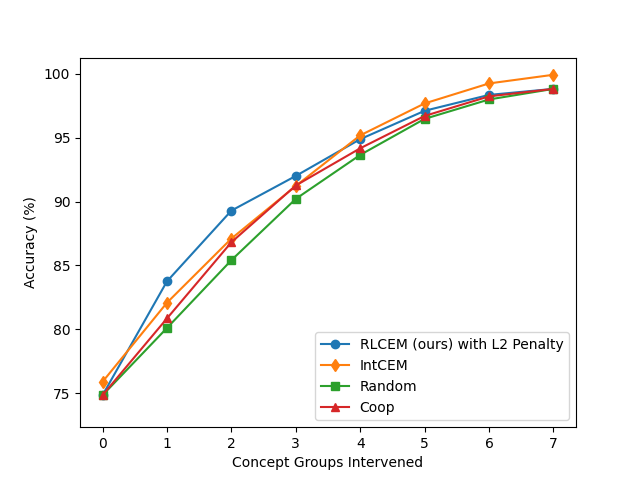
\includegraphics[width=0.9\textwidth]{figs/evaluation/cub_rlcem_performance_l2.png}
    \caption{
        Intervention Accuracy (\%) of RLCEM intervention
        policy trained with $\ell_2$ Penalty, compared to existing intervention policies on CUB.
    }
    \label{fig:cub-rlcem_performance-l2}
\end{figure}

% In Table~\ref{table:cub-performance-l2},
% we tabulate the intervention accuracies 
% of RLCEM compared to other greedy policies 
% across quartiles of interventions performed.
% For each quartile, the accuracy is calculated by 
% linearly interpolating the two points around the quartile
% boundary. For example, to calculate 
% the 50\% quartiles, we take the mean of the 
% intervention accuracy with 3 and 4 groups intervened.
% From the results we can see that RLCEM only outperforms
% IntCEM and the other policies at one quartile, and that the 
% RLCEM results have a very high standard deviation.

% \begin{table}[!ht]
%     \centering
%     \renewcommand{\arraystretch}{1.5}
%     \begin{tabular}{c|ccccc}
%         \begin{tabular}{@{}c@{}}Concept Groups \\ Intervened\end{tabular} & RLCEM (Ours) & IntCEM & CooP & Random \\
%     \hline
%     % $0\%$ & $\mathbf{88.2} \pm 0.3$ & $\mathbf{88.24} \pm 0.09$ & $\mathbf{88.24} \pm 0.09$ & $\mathbf{88.24} \pm 0.09$ \\
%     % $25\%$ & $\mathbf{91.1} \pm 0.4$ & $\mathbf{90.7} \pm 0.3$ & $88.7 \pm 0.2$ & $89.55 \pm 0.08$ \\
%     % $50\%$ & $\mathbf{93.2} \pm 0.2$ & $91.1 \pm 0.3$ & $91.1 \pm 0.2$ & $91.24 \pm 0.07$ \\
%     % $75\%$ & $\mathbf{94.0} \pm 0.2$ & $91.7 \pm 0.3$ & $93.4 \pm 0.2$ & $92.7 \pm 0.2$ \\
%     % $100\%$ & $\mathbf{94.5} \pm 0.4$ & $\mathbf{94.2} \pm 0.3$ & $\mathbf{94.2} \pm 0.3$ & $\mathbf{94.2} \pm 0.3$ \\
%     $0\%$ & $\mathbf{74} \pm 1$ & $\mathbf{75} \pm 1$ & $\mathbf{74} \pm 1$ & $\mathbf{74} \pm 1$ \\
%     $25\%$ & $\mathbf{87} \pm 2$ & $\mathbf{85} \pm 1$ & $\mathbf{85} \pm 3$ & $84 \pm 2$ \\
%     $50\%$ & $\mathbf{93} \pm 2$ & $\mathbf{93} \pm 1$ & $\mathbf{92} \pm 3$ & $\mathbf{91} \pm 3$ \\
%     $75\%$ & $97 \pm 2$ & $\mathbf{98.1} \pm 0.7$ & $97 \pm 2$ & $96 \pm 2$ \\
%     $100\%$ & $98.8 \pm 0.8$ & $\mathbf{99.9} \pm 0.1$ & $98.8 \pm 0.8$ & $98.8 \pm 0.8$ \\
%     \end{tabular}
%     \caption{Intervention Accuracy (\%) of RLCEM intervention
%     policy trained with L2 Penalty, compared to existing intervention policies on CUB.
%     We display the results across quartiles of interventions performed.
%     Higher is better. We highlight the 
%     best performing policy in each row and values within 1 standard deviation.
%     }
%     \label{table:cub-performance-l2}
% \end{table}

Therefore, we cannot conclude that RLCEM is better than the greedy
intervention policies in CUB. Penalizing large outputs 
in the AC Flow model results in more similar output values for the likelihood
of different concepts, and the approximated information gain is no longer
accurate and cannot act as a useful reward to guide the RL agent to make 
the optimal interventions, and the RL agent struggles to learn a good intervention policy.
The large standard deviation also shows that this method is not robust
and the performance can greatly differ.
This shows that this method, while showing promising results on MNIST-ADD on itself,
is not robust and widely applicable as 
there is no simple solution to the large likelihoods outputted by the surrogate model. Future work can investigate better methods
to constrain the size of the likelihoods outputted by the surrogate model to improve robustness.

\subsection{Back to MNIST-ADD}\label{eval:back-to-mnist}
While the $\ell_2$ penalty solves the issues 
related to large likelihoods, we show that 
it harms the training of the RL agent,
and we further demonstrate this by
investigating the performance of RLCEM on MNIST-ADD with and without
this $\ell_2$ penalty.
As shown in Figure~\ref{fig:mnist-rlcem-performance-l2},
after adding a $\ell_2$ Penalty to the AC Flow model,
while still slightly better than Random, the intervention performance of RLCEM significantly decreases.
This confirms that adding the $\ell_2$ Penalty
to the AC Flow model worsens the intervention performance of 
RLCEM, resulting in poor performing 
AC Flow models.
This leads to the inconsistent and poorer
intervention performances.

\begin{figure}[!h]
    \centering
    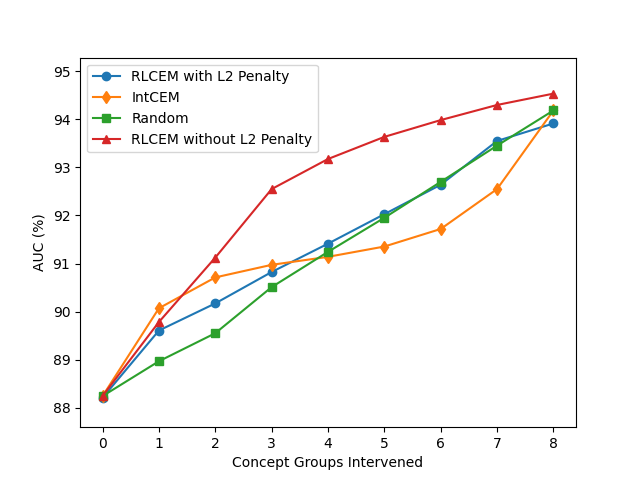
\includegraphics[width=0.9\textwidth]{figs/evaluation/mnist_rlcem_performance_l2.png}
    \caption{
        Intervention AUC (\%) of RLCEM trained with and without an $\ell_2$ Penalty (for the used AC Flow model).
        We also include IntCEM and Random for reference.
    }
    \label{fig:mnist-rlcem-performance-l2}
\end{figure}



\section{Limitations}\label{eval:limitations}
While we have shown that RLCEM can learn a non-greedy intervention 
policy that outperforms existing greedy intervention
policies, it also has its drawbacks. Most notably the largest
drawback is its inconsistent performances which are dependent
on the output of the AC Flow model. When we add an $\ell_2$ Penalty
to train the AC Flow model, it then struggles to learn to 
output accurate conditional likelihood. This then affects the RL 
agent, which struggles to learn the optimal interventions with a 


Another limitation of RLCEM is its time complexity.
Table~\ref{table:training-times} shows the per-epoch
training times of RLCEM. As mentioned in Section~\ref{method:limitations}
RLCEM has a training time complexity of $O(n^2k)$ compared
to IntCEM's $O(n)$, which makes it not scalable for tasks
with large concepts. This is reflected by the much higher
per-epoch training time of RLCEM compared to IntCEM, especially
to CUB where one epoch of RLCEM takes more than ten times longer
than IntCEM, as CUB has a large number of concepts
. This number further increases if we want to increase 
the number of budgets sampled for training for each mini-batch.

\begin{table}[!ht]
    \renewcommand{\arraystretch}{1.5}
    \centering
    \begin{tabular}{c|cc}
        Task & RLCEM & IntCEM \\
        \hline
        MNIST-ADD & $77.8 \pm 0.8$ & $13.96 \pm 0.04$ \\
        CUB & $610 \pm 30$ & $44 \pm 5$ 
        
    \end{tabular}
    \caption{Per epoch Training Time in seconds of RLCEM vs IntCEM.}
    \label{table:training-times}
\end{table}

Lastly, RLCEM is also impacted by concept-incompleteness. As mentioned in Section~\ref{background:cem},
the concept embeddings used by CEM can encode
extra information representing other concepts within the concept embeddings.
This weakens the performance of the AC Flow models as they are trained purely on the concept annotations, and concept incompleteness makes it so the approximated distribution of concepts 
do not accurately represent the distribution of concepts embeddings.

\section{Summary}
In this chapter, we have successfully evaluated the performance
of RLCEM against existing greedy intervention policies 
and random.
We have shown that RLCEM outperforms the SOTA 
greedy intervention
policies on MNIST-ADD, achieving similar or better
intervention performance with 25\% less interventions performed.
However, this method is not robust as seen from its
failures in learning a good non-greedy intervention policy from the 
CUB task. The method is highly dependent on the quality of 
outputs from the pre-trained AC Flow model, which in turn can
vary
from task to task.
\end{document}